\input templates/header

% \usepackage{epigraph}
 \usepackage{tikz}
% \usepackage{multicol}
\usepackage{xmpmulti}
\usepackage{listings}


\lstset{
  basicstyle=\ttfamily,
  columns=fullflexible,
  keywordstyle=\color{red}\bfseries,
  commentstyle=\color{blue},
  showstringspaces=false,
}

\newcommand{\Sum}{\mathit{sum}}


\title[ASD - Strutture dati]{\textbf{Algoritmi e Strutture Dati}\\[24pt]Strutture di dati}

\graphicspath{{figs/03/}}

\begin{document}

%-------------------------------------------------------------------------
\FrameTitle{}

%-------------------------------------------------------------------------
\FrameContent

\section{Strutture dati astratte}

\subsection{Definizioni}

%-------------------------------------------------------------------------
\begin{frame}{Introduzione}

\begin{myboxtitle}[Dato]
In un linguaggio di programmazione, un dato è un valore che una variabile può assumere
\end{myboxtitle}

\begin{myboxtitle}[Tipo di dato astratto]
Un modello matematico, dato da una collezione di valori e un insieme di operazioni ammesse su questi valori
\end{myboxtitle}

\begin{myboxtitle}[Tipi di dato primitivi]
\BI
\item Forniti direttamente dal linguaggio
\item Esempi: int (\texttt{+,-,*,/, \%}), boolean (\texttt{!, \&\&, ||})
\EI
\end{myboxtitle}

\end{frame}


%-------------------------------------------------------------------------
\begin{frame}{Tipi di dati}
  
\begin{myboxtitle}[“Specifica” e “implementazione” di un tipo di dato astratto]
\BI
\item \alert{Specifica}: “manuale d'uso”, nasconde i dettagli implementativi all'utilizzatore
\item \alert{Implementazione}: realizzazione vera e propria
\EI
\end{myboxtitle}

\begin{myboxtitle}[Esempi]
\begin{center}
\begin{tabular}{|P{3cm}|P{7cm}|}
\hline
\textbf{Specifica} & \textbf{Implementazione} \\
\hline
Numeri reali & IEEE-754 \\
\hline
Pile & Pile basate su vettori \newline Pile basate su puntatori \\
\hline
Code & Code basate su vettori circolari \newline Code basate su puntatori \\
\hline
\end{tabular}
\end{center}
\end{myboxtitle}
  
\end{frame}

%-------------------------------------------------------------------------
\begin{frame}{Strutture di dati}

\vspace{-6pt}
\begin{myboxtitle}[Strutture di dati]
Le strutture di dati sono collezioni di dati, caratterizzate più
dall'organizzazione della collezione piuttosto che dal tipo dei dati contenuti.
\end{myboxtitle}

\begin{myboxtitle}[Come caratterizzare le strutture dati]
\BI
\item un insieme di operatori che permettono di manipolare la struttura 
\item un modo sistematico di organizzare l'insieme dei dati
\EI
\end{myboxtitle}

\begin{myboxtitle}[Alcune tipologie di strutture di dati]
\BI
\item \alert{Lineari} / \alert{Non lineari} (presenza di una sequenza)
\item \alert{Statiche} / \alert{Dinamiche} (variazione di dimensione, contenuto)
\item \alert{Omogenee} / \alert{Disomogenee} (dati contenuti) 
\EI
\end{myboxtitle}

\end{frame}

%-------------------------------------------------------------------------
\begin{frame}{Strutture di dati}
  
{\footnotesize
\begin{tabular}{|P{1.5cm}|P{2.9cm}|P{2.9cm}|P{2.9cm}|}
\hline
\textbf{Tipo} & \textbf{Java} & \textbf{C++} & \textbf{Python} \\
\hline
\alert{Sequenze} & \textcolor{DarkRed}{\texttt{List}, \texttt{Queue}, \texttt{Deque}}
\newline \texttt{LinkedList}, \texttt{ArrayList}, \texttt{Stack}, \texttt{ArrayDeque}
&  
\texttt{list}, \texttt{forward\_list} \newline \texttt{vector} \newline \texttt{stack} \newline \texttt{queue}, \texttt{deque} &
\texttt{list} \newline \texttt{tuple} \\
\hline
\alert{Insiemi} & \textcolor{DarkRed}{\texttt{Set}} \newline\texttt{TreeSet}, \texttt{HashSet}, \texttt{LinkedHashSet} & \texttt{set} \newline \texttt{unordered\_set} & \texttt{set}, \texttt{frozenset}  \\
\hline
\alert{Dizionari} & \textcolor{DarkRed}{\texttt{Map}} \newline \texttt{HashTree}, \texttt{HashMap}, \texttt{LinkedHashMap} & \texttt{map} \newline \texttt{unordered\_map} & \texttt{dict} \\
\hline 
\alert{Alberi}\newline & ~\newline- & ~\newline- & ~\newline- \\
\hline
\alert{Grafi}\newline & ~\newline- & ~\newline- & ~\newline- \\
\hline
\end{tabular}
}

\end{frame}

\subsection{Sequenza}

%-------------------------------------------------------------------------
\begin{frame}{Sequenza}

\begin{myboxtitle}[Sequenza]
Una struttura dati \alert{dinamica}, \alert{lineare} che rappresenta una 
sequenza \alert{ordinata} di valori, dove un valore può comparire
più di una volta.
\BI
\item L'ordine all'interno della sequenza è importante
\EI
\end{myboxtitle}

\begin{myboxtitle}[Operazioni ammesse]
\BI
\item
Data la posizione, è possibile aggiungere / togliere elementi 
\BI
\item $s = s_1, s_2, \ldots, s_n$
\item l'elemento $s_i$ è in posizione $\mathit{pos}_i$
\item esistono le posizioni (fittizie) $\mathit{pos}_0, \mathit{pos}_{n+1}$
\EI
\item \EE possibile accedere direttamente alla testa/coda
\item \EE possibile accedere sequenzialmente a tutti gli altri elementi
\EI
\end{myboxtitle}
  
\end{frame}


%-------------------------------------------------------------------------
\begin{frame}[shrink=10]{Sequenza -- Specifica}

\vspace{-12pt}
\begin{Procedure}
\caption[A]{\Sequence}

\BlankLine
\% Restituisce \TRUE\ se la sequenza è vuota\;
\alert{\BOOLEAN\ \listempty()\;}

\BlankLine
\% Restituisce \TRUE\ se $p$ è uguale a $\Pos_0$ oppure a $\Pos_{n+1}$\;
\alert{\BOOLEAN\ \listend($\Postype\ p$)\;}

\BlankLine
\% Restituisce la posizione del primo elemento\;
\alert{\Postype\ \listhead()\;}

\BlankLine
\% Restituisce la posizione dell'ultimo elemento\;
\alert{\Postype\ \listtail()\;}

\BlankLine
\% Restituisce la posizione dell'elemento che segue $p$\;
\alert{\Postype\ \listsucc($\Postype\ p$)\;}

\BlankLine
\% Restituisce la posizione dell'elemento che precede $p$\;
\alert{\Postype\ \listpred($\Postype\ p$)\;}

\end{Procedure}
\end{frame}

%-------------------------------------------------------------------------
\begin{frame}[shrink=10]{Sequenza -- Specifica}

\vspace{-12pt}
\begin{Procedure}
\caption[A]{\Sequence (continua)}

\% Inserisce l'elemento $v$ di tipo $\Item$ nella posizione $p$.\; 
\% Restituisce la posizione del nuovo elemento, che diviene il predecessore di $p$\;
\alert{\Postype\ \listinsert($\Postype\ p,\ \Item\ v$)\;}

\BlankLine
\% Rimuove l'elemento contenuto nella posizione $p$.\;
\% Restituisce la posizione del successore di $p$, \;
\% che diviene successore del predecessore di $p$\;
\alert{\Postype\ \listRemove($\Postype\ p$)\;}

\BlankLine
\% Legge l'elemento di tipo $\Item$ contenuto nella posizione $p$\;
\alert{\Item \listread($\Postype\ p$)\;}

\BlankLine
\% Scrive l'elemento $v$ di tipo $\Item$ nella posizione $p$\;
\alert{\listwrite($\Postype\ p,\ \Item\ v$)\;}

\end{Procedure}

\end{frame}

\begin{frame}[fragile,shrink=10]{Sequenza}


\vspace{-6pt}
\begin{myboxtitle}[Java]
\begin{lstlisting}[language=Java]
List<String> lista = new LinkedList<String>();
lista.add("two"); 
lista.addFirst("one");
lista.addLast("three");
\end{lstlisting}
\alert{Result}: \texttt{['one', 'two', 'three']}
\end{myboxtitle}

\vspace{-6pt}
\begin{columns}[T]
\begin{column}{0.40\textwidth}
\begin{myboxtitle}[C++]
\begin{lstlisting}[language=C++]
std::list<int> lista;
lista.push_front(2);
lista.push_front(1);
lista.push_back(3);
\end{lstlisting}
\alert{Result}: \texttt{[1,2,3]}
\end{myboxtitle}
\end{column}
\begin{column}{0.56\textwidth}

%}
%{
\begin{myboxtitle}[Python]
\begin{lstlisting}[language=python]
lista = ["one", "three"]
lista.insert(1, "two")
\end{lstlisting}
\alert{Result}: \texttt{[ 'one', 'two', 'three' ]}
\end{myboxtitle}
\end{column}
\end{columns}
%}



\end{frame}



\subsection{Insiemi}

%-------------------------------------------------------------------------
\begin{frame}[shrink=5]{Insiemi}
  
\vspace{-6pt}
\begin{myboxtitle}[Insieme]
Una struttura dati \alert{dinamica}, \alert{non lineare} che memorizza una \alert{collezione non ordinata di 
elementi} senza valori ripetuti.
\BI
\item L'ordinamento fra elementi è dato dall'eventuale relazione d'ordine definita sul tipo degli elementi stessi
\EI
\end{myboxtitle}

\begin{myboxtitle}[Operazioni ammesse]

\TwoCols{
\BIL
\item Operazioni base: 
\BI
\item inserimento
\item cancellazione
\item verifica contenimento
\EI
\item Operazioni di ordinamento
\BI
\item Massimo
\item Minimo
\EI
\EIL
}{
\BI
\item Operazioni insiemistiche:
\BI
\item unione
\item interesezione
\item differenza
\EI
\item Iteratori:
\BI
\item \textbf{foreach}\ $x \in S$ \textbf{do}
\EI
\EI
}
\end{myboxtitle}

\end{frame}


%-------------------------------------------------------------------------
\begin{frame}[shrink=12]{Insiemi -- Specifica}

\vspace{-12pt}
\begin{Procedure}
\caption{\Set}

\% Restituisce la cardinalità dell'insieme\;
\alert{\INTEGER\ $=ize()$}
\BlankLine

\% Restituisce \TRUE se $x$ è contenuto nell'insieme\;
\alert{\BOOLEAN\ $\setcontains(\Item\ x)$}
\BlankLine

\% Inserisce $x$ nell'insieme, se non già presente\;
\alert{$\setinsert(\Item\ x)$}
\BlankLine

\% Rimuove $x$ dall'insieme, se presente\;
\alert{$\setremove(\Item\ x)$}
\BlankLine

\% Restituisce un nuovo insieme che è l'unione di $A$ e $B$\;
\alert{\Set \setunion(\Set\ $A$, \Set $B$)}
\BlankLine

\% Restituisce un nuovo insieme che è l'intersezione di $A$ e $B$\;
\alert{\Set \setintersection(\Set $A$, \Set $B$)}
\BlankLine

\% Restituisce un nuovo insieme che è la differenza di $A$ e $B$\;
\alert{\Set \setdifference(\Set $A$, \Set $B$)}
\end{Procedure}
  
\end{frame}

\begin{frame}[fragile,shrink=18]{Insiemi}

\vspace{-6pt}
\begin{myboxtitle}[Java]
\vspace{-6pt}
\begin{lstlisting}[language=Java]
Set<String> docenti = new TreeSet<>();
docenti.add("Alberto");
docenti.add("Cristian");
docenti.add("Alessio");
\end{lstlisting}
\alert{Result}: \texttt{\{ "Alberto", "Alessio", "Cristian" \}}
\end{myboxtitle}

\vspace{-6pt}
\begin{columns}[T]
\begin{column}{0.48\textwidth}
\begin{myboxtitle}[C++]
\vspace{-6pt}
\begin{lstlisting}[language=C++]
std::set<std::string> frutta;
frutta.insert("mele");
frutta.insert("pere");
frutta.insert("banane");
frutta.insert("mele");
frutta.remove("mele")
\end{lstlisting}
\alert{Result}: \texttt{\{ "banane", "pere" \}}
\end{myboxtitle}
\end{column}
\begin{column}{0.48\textwidth}
\begin{myboxtitle}[Python]
\vspace{-6pt}
\begin{lstlisting}[language=python]
items = { "rock", "paper", 
   "scissors", "rock" } 
print(items) 
print("Spock" in items) 
print("lizard" not in items) 
\end{lstlisting}
\alert{Result}:\\
\texttt{\{ "rock", "paper", "scissors" \}} \\
\texttt{False} \\
\texttt{True} 
\end{myboxtitle}
\end{column}
\end{columns}

\end{frame}


\subsection{Dizionari}


%-------------------------------------------------------------------------
\begin{frame}{Dizionari}
  
\begin{myboxtitle}[Dizionario]
Struttura dati che rappresenta il concetto matematico di \alert{relazione univoca}
$R: D \rightarrow C$, o associazione chiave-valore.
\BI
\item Insieme $D$ è il \alert{dominio} (elementi detti \alert{chiavi})
\item Insieme $C$ è il \alert{codominio} (elementi detti \alert{valori})
\EI
\end{myboxtitle}
  
\begin{myboxtitle}[Operazioni ammesse]
\BI
\item Ottenere il valore associato ad una particolare chiave (se presente), o \textbf{nil} se assente
\item Inserire una nuova associazione chiave-valore, cancellando eventuali associazioni precedenti per la stessa chiave 
\item Rimuovere un'associazione chiave-valore esistente  
\EI
\end{myboxtitle}

\end{frame}

%-------------------------------------------------------------------------
\begin{frame}{Dizionari -- Specifica}
  
\begin{Procedure}
\caption[A]{\Dictionary}
\BlankLine

\% Restituisce il valore associato alla chiave $k$ se presente, \Nil altrimenti\;
\alert{\Item\ \dictlookup(\Item\ $k$)\;}
\BlankLine

\% Associa il valore $v$ alla chiave $k$\;
\alert{\setinsert(\Item\ $k$, \Item\ $v$)\;}
\BlankLine

\% Rimuove l'associazione della chiave $k$\;
\alert{\setremove(\Item\ $k$)\;}
\end{Procedure}
  
  
\end{frame}


\begin{frame}[fragile, shrink=5]{Array associativi, mappe e dizionari}

\small
\vspace{-6pt}
\begin{myboxtitle}[Java]
\begin{lstlisting}[language=java]  
Map<String, String> capoluoghi = new HashMap<>();
capoluoghi.put("Toscana", "Firenze");
capoluoghi.put("Lombardia", "Milano");
capoluoghi.put("Sardegna", "Cagliari");
\end{lstlisting}
\end{myboxtitle}

\vspace{-6pt}
\begin{columns}
\begin{column}{0.62\textwidth}
\begin{myboxtitle}[C++]
\begin{lstlisting}[language=c++]  
std::map<std::string, int> wordcounts;
std::string s;

while (std::cin >> s && s != "end")
  ++wordcounts[s];
\end{lstlisting}
\end{myboxtitle}
\end{column}
\begin{column}{0.34\textwidth}
\begin{myboxtitle}[Python]
\begin{lstlisting}[language=python]  
v = {} 
v[10] = 5 
v["alberto"] = 42 
v[10]+v["alberto"] 
\end{lstlisting}
\alert{Result}: \texttt{47}
\end{myboxtitle}
\end{column}
\end{columns}


\end{frame}

\subsection{Alberi e grafi}

%-------------------------------------------------------------------------
\begin{frame}{Alberi e grafi}

\begin{myboxtitle}[Alberi ordinati]
\BI
\item Un \alert{albero ordinato} è dato da un insieme finito di elementi detti \alert{nodi}
\item Uno di questi nodi è designato come \alert{radice}
\item I rimanenti nodi, se esistono sono partizionati in insiemi \alert{ordinati}
e \alert{disgiunti}, anch'essi alberi ordinati
\EI
\end{myboxtitle}

\IG{0.45}{alberi-crop.pdf}
  

\end{frame}

%-------------------------------------------------------------------------
\begin{frame}<handout:0>[noframenumbering]{Alberi e grafi}
\IG{1.0}{paperi.jpg}
\end{frame}

%-------------------------------------------------------------------------
\begin{frame}{Alberi e grafi}

\TwoColsCustom{0.68}{0.28}{
\begin{myboxtitle}[Grafi]
La struttura dati grafo è composta da:
\BI
\item un insieme di elementi detti \alert{nodi} o \alert{vertici} 
\item un insieme di coppie (ordinate oppure no) di nodi detti \alert{archi}
\EI
\end{myboxtitle}
}{
\vspace{-6pt}
\begin{center}
\IG{1.0}{grafi-crop.pdf}
\end{center}
}
\begin{myboxtitle}[Operazioni]
\BI
\item Tutte le operazioni su alberi e grafi ruotano attorno alla possibilità di 
effettuare \alert{visite} su di essi
\item Specifica completa più avanti
\EI
\end{myboxtitle}

\end{frame}

%-------------------------------------------------------------------------
\begin{frame}{Commenti}

\BIL
\item \alert{Concetti di sequenza, insieme, dizionario sono collegati}
\BI
\item  Insieme delle chiavi / insieme dei valori
\item  Scorrere la sequenza di tutte le chiavi
\EI
\item \alert{Alcune realizzazioni sono "naturali"}
\BI
\item Sequenza $\leftrightarrow$ lista
\item Albero astratto $\leftrightarrow$ albero basato su puntatori
\EI
\item \alert{Esistono tuttavia realizzazioni alternative}
\BI
\item Insieme come vettore booleano
\item Albero come vettore dei padri
\EI
\item \alert{La scelta della struttura di dati ha riflessi sull'efficienza e sulle operazioni ammesse}
\BI
\item Dizionario come hash table: lookup $O(1)$, ricerca minimo $O(n)$
\item Dizionario come albero: lookup $O(\log n)$, ricerca minimo $O(1)$
\EI
\EIL

\end{frame}

\section{Implementazione strutture dati elementari}

\subsection{Lista}

\begin{frame}{Lista}

\vspace{-6pt}
\begin{myboxtitle}[Lista (Linked List)]
Una sequenza di nodi, contenenti dati arbitrari e 1-2 puntatori all'elemento successivo e/o precedente.
\end{myboxtitle}

\begin{myboxtitle}[Note]
\BI
\item Contiguità nella lista $\not \Rightarrow$ contiguità nella memoria
\item Tutte le operazioni hanno costo $O(1)$
\EI
\end{myboxtitle}


\begin{myboxtitle}[Possibili implementazioni]
\BI
\item \alert{Bidirezionale} / \alert{Monodirezionale}
\item \alert{Con sentinella} / \alert{Senza sentinella}
\item \alert{Circolare} / \alert{Non circolare}  
\EI
\end{myboxtitle}

\end{frame}

\begin{frame}{Lista}
  
\begin{center}
\IG{0.8}{lista-crop.pdf}
\end{center}
\end{frame}


\begin{frame}[shrink=40]{Lista bidirezionale con sentinella}

\vspace{-12pt}
\begin{Procedure}
\caption[A]{\List}
\begin{multicols}{2}

\List\ \Pred\REMR{Predecessore}
\List\ \Succ\REMR{Successore}
\Item\ \Valuevar\REMR{Elemento}
\BlankLine  

\PROCEDURE{\List\ \listconstructor()}
{
  $\List\ t = \NEW\ \List$\;
  $t.\Pred = t$\;
  $t.\Succ = t$\;
  \Return $t$\;
}
\BlankLine  

\BOOLEAN\ \PROCEDURE{\listempty()}
{
  \Return\ \Pred = \Succ = \THIS\;
}
\BlankLine  

\Postype\ \PROCEDURE{\listhead()}
{
  \Return\ \Succ\;
}
\BlankLine  
  
\Postype\ \PROCEDURE{\listtail()}
{
  \Return\ \Pred\;
}
\BlankLine  
  
\Postype\ \PROCEDURE{\listsucc(\Postype\ $p$)}
{
  \Return\ $p.\Succ$\;
}
\BlankLine  

\Postype\ \PROCEDURE{\listpred(\Postype\ $p$)}
{
  \Return\ $p.\Pred$\;
}

\BOOLEAN \PROCEDURE{\listend(\Postype\ $p$)}
{
  \Return\ $(p = \THIS)$\;
}
\BlankLine  

\Item\ \PROCEDURE{\listread(\Postype\ $p$)}
{
  \Return\ $p.\Valuevar$\;
}
\BlankLine  

\PROCEDURE{\listwrite(\Postype\ $p$, \Item\ $v$)}
{
  $p.\Valuevar = v$\;
}
\BlankLine  

\Postype\ \PROCEDURE{\listinsert(\Postype\ $p$, \Item\ $v$)}
{
  $\List\ t = \listconstructor()$\;
  $t.\Valuevar = v$\;
  $t.\Pred = p.\Pred$ 
  \;
  $p.\Pred.\Succ = t$\;
  $t.\Succ = p$
  \;
  $p.\Pred = t$\;
  \Return $t$;
}
\BlankLine  
  
\Postype\ \PROCEDURE{\listremove(\Postype\ $p$)}
{
  $p.\Pred.\Succ = p.\Succ$
  \;
  $p.\Succ.\Pred = p.\Pred$
  \;
  $\List\ t = p.\Succ$\;
  \DELETE\ $p$\;
  \Return\ $t$;
}
\end{multicols}
\end{Procedure}
\tiny{\List e \Postype sono tipi equivalenti}
\end{frame}


\begin{frame}[fragile,shrink=3]{Lista bidirezionale senza sentinella -- Java}

\vspace{-12pt}
\begin{lstlisting}[language=java]
class Pos {

  Pos succ;              /** Next element of the list */
  Pos pred;              /** Previous element of the list */
  Object v;              /** Value */

  Pos(Object v) {
    succ = pred = null;
    this.v = v;
  }
}
\end{lstlisting}
\end{frame}

\begin{frame}[fragile,shrink=10]{Lista bidirezionale senza sentinella -- Java}

\vspace{-12pt}
\begin{lstlisting}[language=java]
public class List {

  private Pos head;      /** First element of the list */
  private Pos tail;      /** Last element of the list */

  public List() { 
    head = tail = null;
  }

  public Pos head()                  { return head; }
  public Pos tail()                  { return tail; }
  public boolean finished(Pos pos)   { return pos == null; }
  public boolean isEmpty()           { return head == null; }
  public Object read(Pos p)          { return p.v; }
  public void write(Pos p, Object v) { p.v = v; }
\end{lstlisting}
\end{frame}

\begin{frame}[fragile,shrink=3]{Lista bidirezionale senza sentinella -- Java}
\vspace{-12pt}
\begin{lstlisting}[language=java]
  public Pos next(Pos pos) { 
    return (pos != null ? pos.succ : null); 
  }

  public Pos prev(Pos pos) { 
    return (pos != null ? pos.pred : null); 
  }

  public void remove(Pos pos) {
    if (pos.pred == null) 
      head = pos.succ;
    else 
      pos.pred.succ = pos.succ;
    if (pos.succ == null) 
      tail = pos.pred;
    else 
      pos.succ.pred = pos.pred;
  }
\end{lstlisting}
\end{frame}


\begin{frame}[fragile,shrink=5]{Lista bidirezionale senza sentinella -- Java}
\vspace{-12pt}
\begin{lstlisting}[language=java]
public Pos insert(Pos pos, Object v) {
Pos t = new Pos(v);
  if (head == null) {
    head = tail = t; // Insert in a emtpy list
  } else if (pos == null) {
    t.pred = tail; // Insert at the end
    tail.succ = t;
    tail = t;
  } else {
    t.pred = pos.pred; // Insert in front of an existing position
    if (t.pred != null)
      t.pred.succ = t;
    else 
      head = t;
      t.succ = pos;
      pos.pred = t;
  }
  return t;
}
\end{lstlisting}
\end{frame}

\begin{frame}<handout:0>[noframenumbering]{Liste}

\IG{1.0}{forgetting.png}
\end{frame}


%%%%%%%%%%%%%%%%%%%%%%%%%%%%%%%%%%%%%%%%%%%%%%%%%%%%%%%%%%%%%%%%%%%%%%%%%%%%%%
\subsection{Pila}

\begin{frame}[shrink=10]{Pila}
\begin{myboxtitle}[Pila (Stack)]
Una struttura dati dinamica, lineare in cui l'elemento rimosso dall'operazione
di cancellazione è predeterminato: “quello che per meno tempo è rimasto
nell'insieme” (\alert{LIFO - Last-in, First-out})
\end{myboxtitle}


\begin{Procedure}
\caption[A]{\Stack}

\% Restituisce \TRUE\ se la pila è vuota\;
\alert{\BOOLEAN\ $\stackempty()$\;}
\BlankLine

\% Inserisce $v$ in cima alla pila\;
\alert{$\stackpush(\Item\ v)$\;}
\BlankLine

\% Estrae l'elemento in cima alla pila e lo restituisce al chiamante\;
\alert{\Item\ $\stackpop()$\;}
\BlankLine

\% Legge l'elemento in cima alla pila\;
\alert{\Item\ $\stacktop()$\;}

\end{Procedure}
\end{frame}

\begin{frame}{Pila}
  
\vspace{-12pt}
\small
\TwoColsCustom{0.72}{0.28}{
  \begin{myboxtitle}[Possibili utilizzi]
  \BIL
    \item Nei linguaggi con procedure:
    \BI
      \item gestione dei record di attivazione
    \EI
    \item Nei linguaggi stack-oriented:
    \BI
      \item le operazioni prendono gli operandi dallo stack e inseriscono  il risultato nello stack
      \item Es: Postscript, Java bytecode
    \EI
  \EIL
  \end{myboxtitle}

  \begin{myboxtitle}[Possibili implementazioni]
  \BIL
    \item Tramite \alert{liste bidirezionali}
    \BI
      \item puntatore all'elemento top
    \EI
    \item Tramite \alert{vettore}
    \BI
      \item dimensione limitata, overhead più basso
    \EI
  \EIL
  \end{myboxtitle}
}{
  \vspace{-6pt}
  \IG{1.0}{pila-lista-crop.pdf}
  \vspace{-6pt}
  \IG{1.0}{pila-vettore-crop.pdf}
}
\end{frame}


\begin{frame}[shrink=5]{Pila basata su vettore -- Pseudocodice}

\begin{Procedure}
\caption{\Stack}
\begin{multicols}{2}

$\Item[\,]\ A$\REMR{Elementi}
$\INTEGER\ \Size$\REMR{Cursore}
$\INTEGER\ \Capacity$\REMR{Dim. massima}
\BlankLine

\PROCEDURE{\Stack\ \stackconstructor(\INTEGER\ $dim$)}
{
  $\Stack\ t = \NEW\ \Stack$\;
  $t.A = \NEW\ \INTEGER[1 \mldots dim]$\;
  $t.\Capacity = dim$\;
  $t.\Size = 0$\;
  \Return $t$\;
}
\BlankLine
  
\PROCEDURE{\Item \stacktop()}
{
  \PRECONDITION: $\Size > 0$\;
  \BlankLine
  \Return $A[\Size]$
}
\columnbreak

\PROCEDURE{\BOOLEAN\ \stackempty()}
{
  \Return $\Size = 0$\;
}
\BlankLine
  
\PROCEDURE{\Item \stackpop()}
{
  \PRECONDITION: $\Size > 0$\;
  \BlankLine
  $\Item\ t = A[\Size]$\;
  $\Size = \Size-1$\;
  \Return $t$\;
}
\BlankLine

\PROCEDURE{\stackpush(\Item\ $v$)}
{
  \PRECONDITION: $\Size < \Capacity$\;
  \BlankLine
  $\Size = \Size+1$\;
  $A[\Size] = v$\; 
}
\BlankLine

\end{multicols}
\BlankLine
\BlankLine

\end{Procedure}


\end{frame}



\begin{frame}[fragile,shrink=5]{Pila basata su vettore -- Java}

\vspace{-6pt}
\begin{lstlisting}[language=java]
public class VectorStack implements Stack {

  /** Vector containing the elements */
  private Object[] A;

  /** Number of elements in the stack */
  private int n;    

  public VectorStack(int dim) {
    n = 0; 
    A = new Object[dim];
  }

  public boolean isEmpty() { 
    return n==0; 
  }
\end{lstlisting}
  
\end{frame}

\begin{frame}[fragile,shrink=5]{Pila basata su vettore -- Java}

\vspace{-6pt}
\begin{lstlisting}[language=java]
  public Object top() { 
    if (n == 0) 
      throw new IllegalStateException("Stack is empty");
    return A[n-1]; 
  }

  public Object pop() {
    if (n == 0) 
      throw new IllegalStateException("Stack is empty");
    return A[--n];
  }

  public void push(Object o) {
    if (n == A.length) 
      throw new IllegalStateException("Stack is full");
    A[n++] = o;
  }
  
}
\end{lstlisting}
  
  
\end{frame}


%%%%%%%%%%%%%%%%%%%%%%%%%%%%%%%%%%%%%%%%%%%%%%%%%%%%%%%%%%%%%%%%%%%%%%%%%%%%%%
\subsection{Coda}

\begin{frame}[shrink=10]{Coda}
  
\begin{myboxtitle}[Coda (Queue)]
Una struttura dati dinamica, lineare in cui l'elemento rimosso dall'operazione
di cancellazione è predeterminato: “quello che per più tempo è rimasto
nell'insieme” (\alert{FIFO - First-in, First-out})
\end{myboxtitle}

\begin{Procedure}
\caption[A]{\Queue}

\% Restituisce \TRUE\ se la coda è vuota\;
\alert{\BOOLEAN\ $\queueempty()$\;}
\BlankLine

\% Inserisce $v$ in fondo alla coda\;
\alert{$\queueinsert(\Item\ v)$\;}
\BlankLine

\% Estrae l'elemento in testa alla coda e lo restituisce al chiamante\;
\alert{\Item\ $\queueremove()$\;}
\BlankLine

\% Legge l'elemento in testa alla coda\;
\alert{\Item\ $\queuetop()$\;}
\end{Procedure}

\begin{tikzpicture}[remember picture,overlay]
    \node[xshift=0cm,yshift=0cm] at (current page.north east){%
    \frame{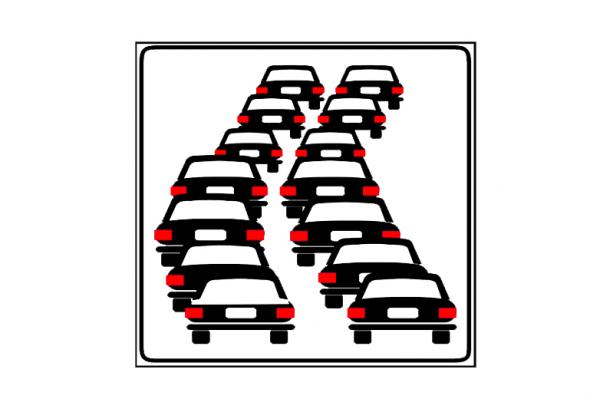
\includegraphics[width=2.2cm]{coda.jpg}}};
\end{tikzpicture}

\end{frame}

\begin{frame}{Coda}
  
\vspace{-12pt}
\TwoColsCustom{0.68}{0.28}{

\begin{myboxtitle}[Possibili utilizzi]
\BI
\item Nei sistemi operativi, i processi in attesa di utilizzare una risorsa vengono gestiti tramite una coda
\item La politica FIFO è \alert{fair}
\EI
\end{myboxtitle}

\begin{myboxtitle}[Possibili implementazioni]
\BIL
\item Tramite \alert{liste monodirezionali}
\BI
\item puntatore head, per estrazione
\item puntatore tail, per inserimento
\EI
\item Tramite \alert{array circolari}
\BI
\item dimensione limitata, overhead più basso
\EI
\EIL
\end{myboxtitle}

}{
\vspace{-6pt}
\IG{1.0}{coda-lista-crop.pdf}
\vspace{-6pt}
\IG{1.0}{circular-23.png}
}

\end{frame}

\begin{frame}{Coda basata su vettore circolare}
\BI
\item La circolarità può essere implementata con l'operazione \alert{modulo}
\item Bisogna prestare attenzione ai problemi di \alert{overflow} (buffer pieno)
\EI

\IG{0.6}{coda-crop.pdf}

\end{frame}

\begin{frame}<handout:0>[noframenumbering]{Coda basata su vettore circolare}

\begin{center}
\multiinclude[<+->][format=png, graphics={width=0.7\textwidth}]{circular}
\end{center}

{\tiny
By MuhannadAjjan [CC BY-SA 4.0] (\url{http://creativecommons.org/licenses/by-sa/4.0})
via Wikimedia Commons
}
\end{frame}


%-------------------------------------------------------------------------
\begin{frame}[shrink=14]{Coda basata su vettore circolare -- Pseudocodice}

\vspace{-12pt}
\begin{Procedure}
\caption{\Queue}
\begin{multicols}{2}
$\Item[\,]\ A$\REMR{Elementi}
$\INTEGER\ \Size$\REMR{Dim. attuale}
$\INTEGER\ \Head$\REMR{Testa}
$\INTEGER\ \Capacity$\REMR{Dim. massima}
\BlankLine

\PROCEDURE{\Queue \queueconstructor(\INTEGER\ $dim$)}
{
  $\Queue\ t = \NEW\ \Queue$\;
  $t.A = \NEW\ \INTEGER[0 \mldots dim-1]$\;
  $t.\Capacity = dim$\;
  $t.\Head = 0$\;
  $t.\Size = 0$\;
  \Return $t$\;
}
\BlankLine

\PROCEDURE{\Item\ \queuetop()}
{
  \PRECONDITION: $\Size > 0$\;
  \BlankLine
  \Return $A[\Head]$
}

\PROCEDURE{\BOOLEAN\ \queueempty()}
{
  \Return $\Size = 0$\;
}
\BlankLine

\PROCEDURE{\Item\ \queueremove()}
{
  \PRECONDITION: $\Size > 0$\;
  \BlankLine
  $\Item\ t = A[\Head]$\;
  $\Head = (\Head+1) \bmod \Capacity$\;
  $\Size = \Size-1$\;
  \Return $t$\;
}
\BlankLine

\PROCEDURE{\queueinsert(\Item\ $v$)}
{
  \PRECONDITION: $\Size < \Capacity$\;
  \BlankLine
  $A[(\Head+\Size) \bmod \Capacity] = v$\; 
  $\Size = \Size+1$\;
}
\end{multicols}
\BlankLine
\BlankLine
\end{Procedure}

\end{frame}



%-------------------------------------------------------------------------
\begin{frame}[fragile,shrink=5]{Coda basata su vettore circolare -- Java}

\begin{lstlisting}[language=Java]
public class VectorQueue implements Queue {

  /** Element vector */
  private Object[] A;

  /** Current number of elements in the queue */
  private int n;    

  /** Top element of the queue */
  private int head;

  public VectorQueue(int dim) {
    n = 0; 
    head = 0;
    A = new Object[dim];
  }

  public boolean isEmpty() {
    return n==0;
  }
\end{lstlisting}

\end{frame}




%-------------------------------------------------------------------------
\begin{frame}[fragile,shrink=5]{Coda basata su vettore circolare -- Java}

\vspace{-12pt}
  \begin{lstlisting}[language=Java]
  public Object top() { 
    if (n == 0) 
      throw new IllegalStateException("Queue is empty");
    return A[head]; 
  }

  public Object dequeue() {
    if (n == 0) 
      throw new IllegalStateException("Queue is empty");
    Object t = A[head];
    head = (head+1) % A.length;
    n = n-1;
    return t;
  }

  public void enqueue(Object v) {
    if (n == A.length) 
      throw new IllegalStateException("Queue is full");
    A[(head+n) % A.length] = v;
    n = n+1;
  }
} 
\end{lstlisting}

\end{frame}

\end{document}
%%%%%%%%%%%%%%%%%%%%%%%%%%%%%%%%%%%%%%%%%%%%%%%%%%%%%%%%%%%%%%%%%%%%%%%%%%


